\documentclass[]{article}
\usepackage{fontspec}
\usepackage{float}
\usepackage[utf8]{inputenc}
\usepackage[portuguese]{babel}
\usepackage[utf8]{inputenc}
\usepackage{amsmath}
\usepackage{subcaption}
\usepackage{mathtools}
\usepackage{graphicx}
\graphicspath{ {./imgs/} }
\usepackage{color}
\usepackage{authblk}
\usepackage{geometry}
\usepackage{indentfirst}
\geometry{
	a4paper,
	total={170mm,257mm},
	left=20mm,
	top=20mm,
}
\usepackage[alf]{abntex2cite}
\setmainfont{Times New Roman}

\title{Banco de Dados}
\author{Lucas Bezerra, Matheus Pessoa, Pedro Guilherme e Vinicius Dias}
\affil{Centro de Ciências Exatas e da Natureza - UFPE\\
	Banco de Dados\\
	Prof. Mário Gomes de Melo}
\date{Outubro 2020}

\begin{document}

\maketitle

\section{Mini-mundo}
Representando a Universidade Federal de Pernambuco no eSport chamado League of Legends, temos a equipe Virtus. Nas partidas, cada jogador assume o papel de um campeão e cada equipe tem como objetivo destruir o Nexus adversário, ao final de cada partida os jogadores possuem um placar de Abates/Mortes/Assistências(AMA). Fora do mundo virtual a equipe é composta por membros, que possuem CPF, nome, curso e data de nascimento. Os mesmos podem ser divididos entre jogadores, capitão e psicólogo, podendo ser mais de um ou nenhum, caso esteja muito ocupado no semestre. Os jogadores tem um psicólogo particular, afim de obter um melhor desempenho. O capitão tem como função liderar os outros jogadores, tendo papel ativo durante as partidas e sendo obrigatoriamente titular. Mais de um jogador pode ter o cargo de capitão, mas apenas um deles exercerá o papel de cada vez. Os demais jogadores são divididos entre titulares ou reservas e fora das partidas um dos jogadores é responsável por treinar toda a equipe. Cada jogador possui um elo, uma classificação, qualificando os jogadores como mais ou menos experientes. Os jogadores também possuem um campeão favorito, uma rota principal, um número de partidas e um nick(nome de usuário). Os jogadores podem participar de campeonatos e partidas ranqueadas. As partidas ranqueadas são jogadas sozinhas ou em grupo e serve para aumentar o seu elo, já os campeonatos são jogados sempre em grupo em busca de títulos.

\section{Requisitos}
\begin{itemize}
    \item O time deseja manter as informações de todos os membros.
    \item Sobre cada membro é importante ter seu CPF, nome, curso e data de nascimento.
    \item Os membros podem ser jogadores, capitão e psicólogo podendo ser mais de um ou nenhum.
    \item Cada jogador tem um psicólogo particular.
    \item O time possui mais de um capitão, mas apenas um exerce o papel de cada vez.
    \item O capitão exercendo o papel é titular e lidera os titulares.
    \item Um jogador será responsável por treinar o time.
    \item Cada jogador possui um elo, campeão favorito(podendo ser mais de um), rota principal, um número de partidas e um nick.
    \item Os jogadores são divididos em titulares e reservas.
    \item Os jogadores  jogam campeonatos e partidas ranqueadas. As partidas ranqueadas são jogadas sozinhas ou em grupo, já os campeonatos são jogados sempre em grupo.
    \item Os jogos tem seu gameID que identifica a partida, o seu resultado, o campeão jogado e o  AMA de cada jogador.
\end{itemize}


\section{Diagrama conceitual}
\begin{figure}[H]
    \centering
    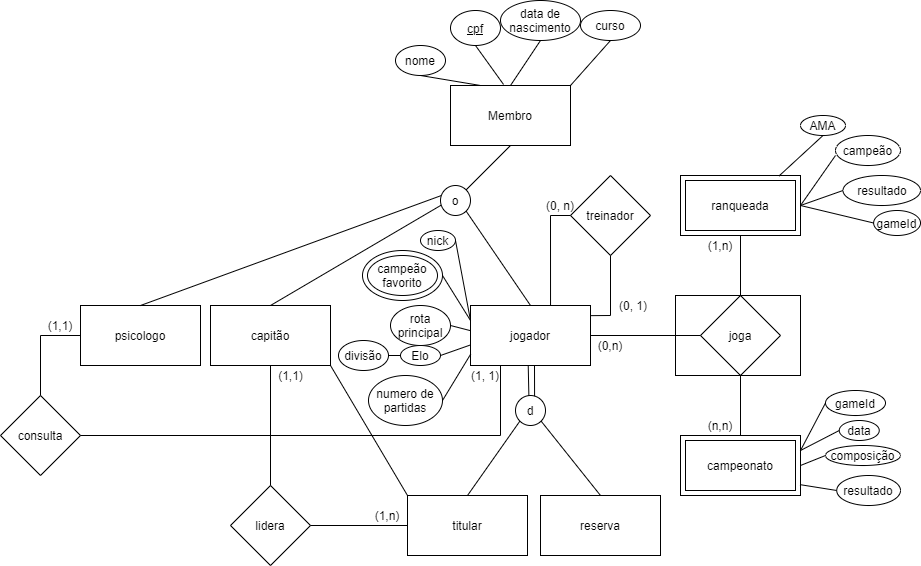
\includegraphics[width=17cm]{conceitual}
\end{figure}

\section{Projeto lógico}
\begin{figure}[H]
    \centering
    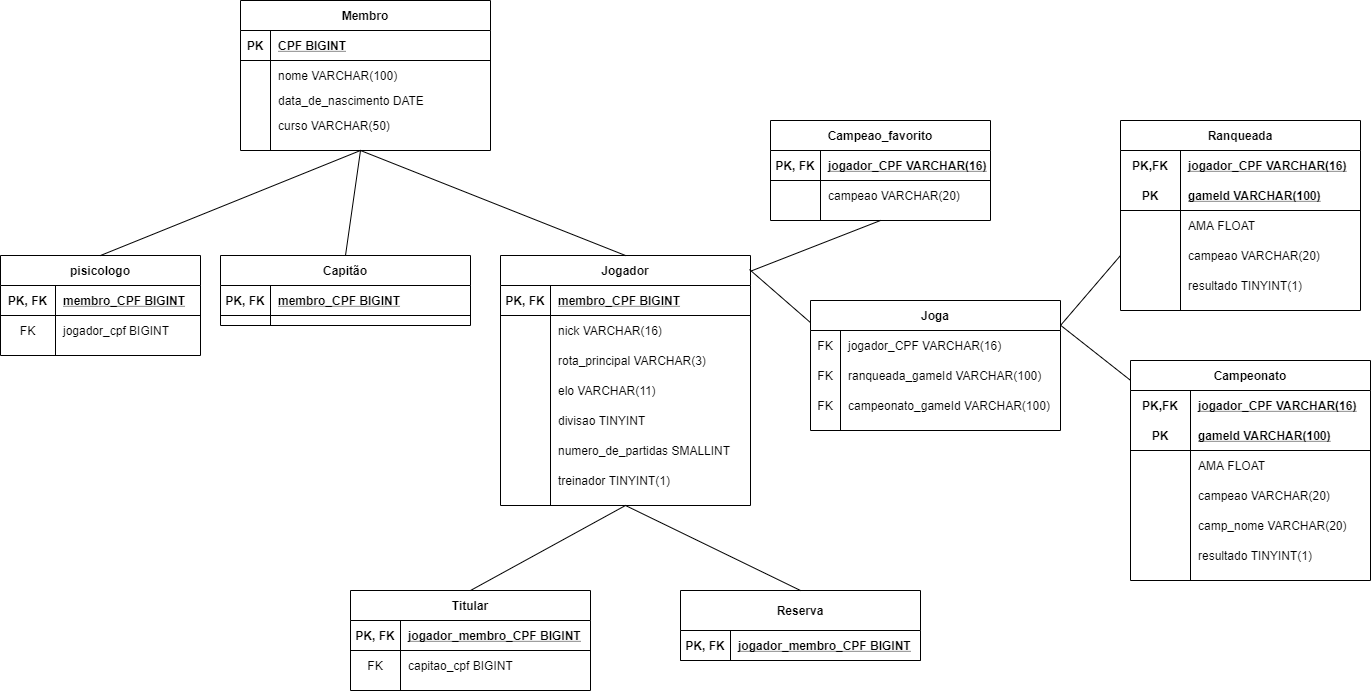
\includegraphics[width=17cm]{logico}
\end{figure}
\end{document}